\begin {itemize}
\item Use Cases
\begin {itemize}
\item {login}\\
Login - Using a provided username and password authenticates the user against details retrieved from an ldap repository
\begin {itemize}
\item Pre-conditions:\\
-could connect to CS data source (LDAP) (implemented in code only, no functional way to test)\\
        -user exists in ldap with provided authentication details (code indicates this is checked by performing a bind to ldap using the provided details)\\
\item Post-conditions:\\
userID returned (not implemented)  
\end {itemize}

\begin{figure}[h!]
  \centering
    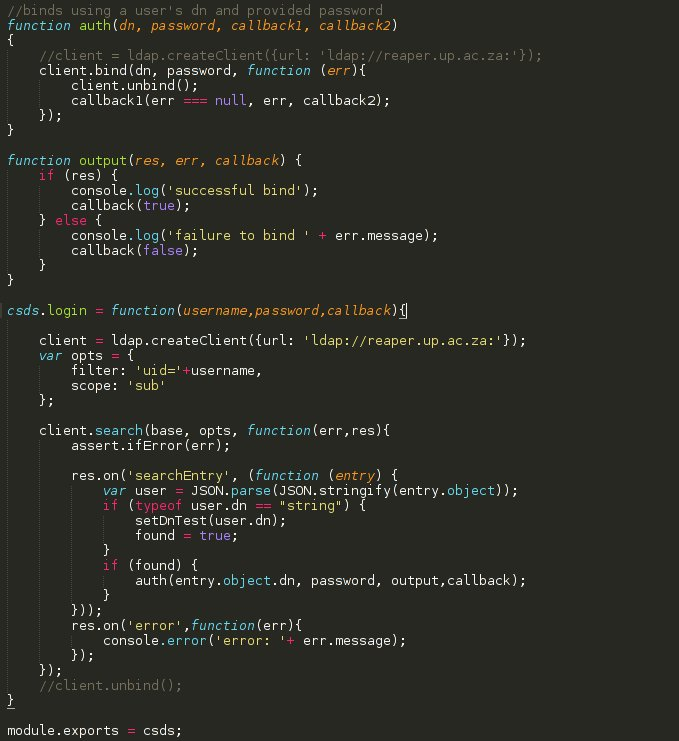
\includegraphics[width=0.85\textwidth]{CSDSLoginCode} 
\end{figure}


\end {itemize}

\begin {itemize}
\item {getUsersRolesForModule}\\
Login - Using a provided username and password authenticates the user against details retrieved from an ldap repository\\
\begin {itemize}
\item Pre-conditions:\\
-could connect to CS data source (LDAP) (implemented in code only, no functional way to test)\\
        -user exists in ldap with provided authentication details (code indicates this is checked by performing a bind to ldap using the provided details)\\
\item Post-conditions:\\
userID returned (not implemented)  
\end {itemize}
	\begin{figure}[h!]
  \centering
    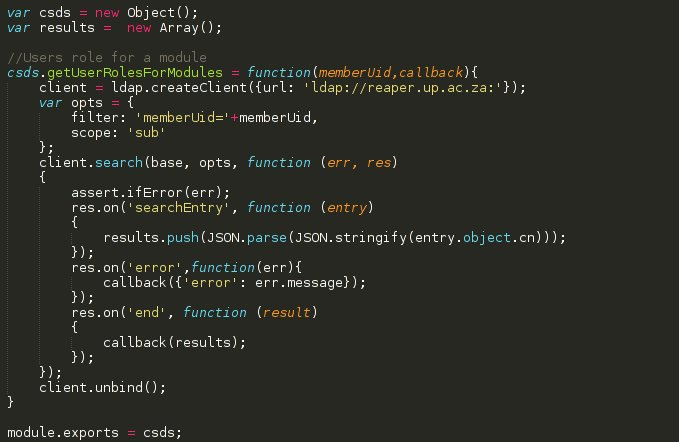
\includegraphics[width=0.85\textwidth]{CSDSUserRolesCode} 
\end{figure}
\end {itemize}

\begin {itemize}
\item {getUsersWithRole}\\
retrieves all users with a particular role for a particular module (no functional way to test)
\begin {itemize}
\item Pre-conditions:\\
-could connect to CS data source (LDAP) (implemented in code only, no functional way to test)\\  
\end {itemize}

\begin{figure}[h!]
  \centering
    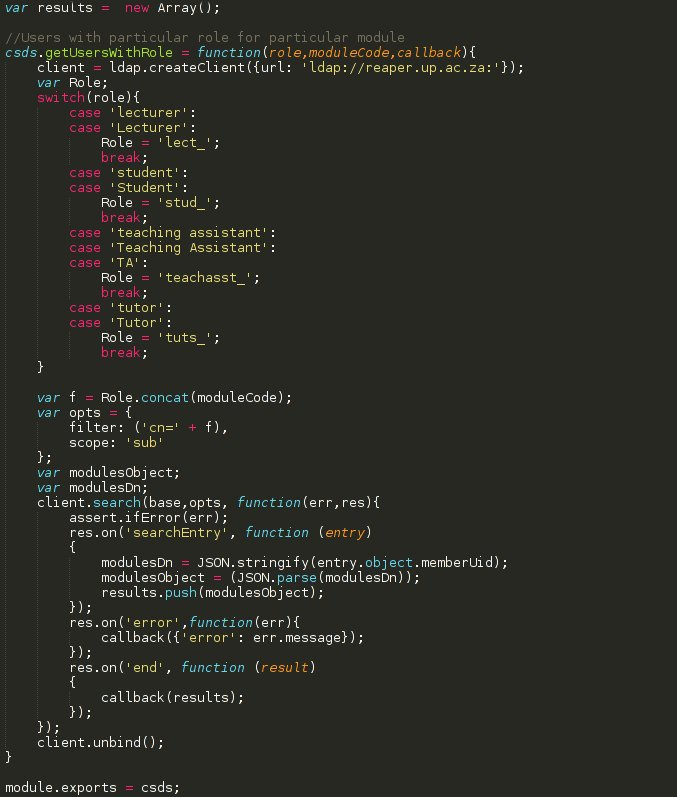
\includegraphics[width=0.85\textwidth]{CSDSGetUsersWithRolesCode} 
\end{figure}


\end {itemize}

\begin {itemize}
\item {getActiveModulesForYear}\\
retrieves all users with a particular role for a particular module (no functional way to test)
\begin {itemize}
\item Pre-conditions:\\
-could connect to CS data source (LDAP) (implemented in code only, no functional way to test)\\  
\end {itemize}
\begin{figure}[h!]
  \centering
    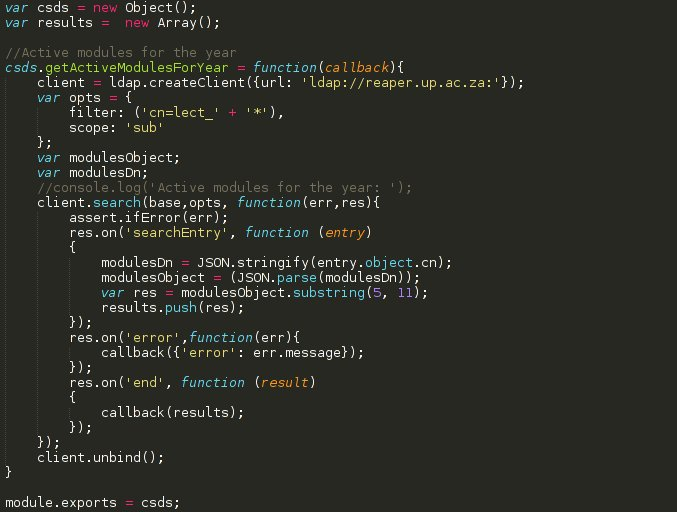
\includegraphics[width=0.85\textwidth]{CSDSGetActiveModulesCode} 
\end{figure}
\end {itemize}

\begin {itemize}
\item {getActiveModulesForYear}\\
retrieves all users with a particular role for a particular module (no functional way to test)
\begin {itemize}
\item Pre-conditions:\\
-could connect to CS data source (LDAP) (implemented in code only, no functional way to test)\\  
\end {itemize}
	
\end {itemize}






\end {itemize}
